\chapter{Umsetzung der Suchmaschine}
In diesem Kapitel wird die Umsetzung der Suchmaschine beschrieben.

Die Suche soll mit Apache Lucene umgesetzt werden. Für die Bedienung genügt in erster Linie ein \gls{cliLabel}.
Aus rechtlichen Gründen, so wie aus Gründen der Verfügbarkeit wird als Grundlage eine \gls{lutLabel}-Übersetzung der Bibel verwendet.

\section{Beschreibung der Suchresultate}
Für jedes Suchresultat soll der Text und die genaue Bibelstelle in folgendem Format ausgegeben werden:\\
"[Text] - `[Buch Abk.], [Kapitel],[Vers]"'

Die Resultate sollen nach einem sinnvollen \gls{glos:rankingLabel} sortiert werden.
Zugunsten einer raschen Erkennbarkeit ist eine farbliche Hervorhebung (Highlighting) der Suchbegriffe in der Resultat-Liste wünschenswert.

\textbf{Beispiel der Resultat-Liste mit Ergebnissen (in originaler Luther Übersetzung):}
\begin{itemize}[noitemsep]
	\item Da wurden sie alle gutes Muts und nahmen auch Speise. - Apg 27,36
	\item Was setzt sich dein Mut gegen Gott, dass du solche Reden aus deinem Munde lässest? - Hiob 15,13
	\item Ein Geduldiger ist besser denn ein Starker, und der seines Mutes Herr ist, denn der Städte gewinnt. - Spr 16,32
\end{itemize}


\section{Optionale Dokumenteinheit}
Der Text von der Luther Bibel muss in \glspl{glos:documentLabel} eingeteilt und zum \gls{glos:indexLabel} hinzugefügt werden.
Die Wahl der Dokumentgrösse hat einen wesentlichen Einfluss auf die Genauigkeit der Resultate.

Zum Beispiel lässt sich die Wichtigkeit der Suchbegriffe im jeweiligen Kontext über den \gls{glos:wordDistanceLabel} gewichten.
Je grösser das \gls{glos:documentLabel} gewählt ist, desto genauer kann das \gls{glos:rankingLabel} berechnet werden.
Gleichzeitig werden Metadaten grundsätzlich pro \gls{glos:documentLabel} gespeichert, also je kleiner ein \gls{glos:documentLabel} gewählt wird, desto genauer kann die Stelle des Auftauchens angezeigt werden.

Diese zwei Anforderungen zeigen einen gewissen Zielkonflikt auf, der folglich optimiert werden muss.

Zuerst wird eine generell passende Dokumentgrösse gesucht, welche dann durch weitere feinere Optimierungen verbessert werden soll.
Dazu muss die Struktur der Bibel, sowie die Grammatik berücksichtigt werden.

\subsection{Möglichkeiten für die Definition der Dokumentgrösse}
Für die Aufteilung der \glspl{glos:documentLabel} gibt es verschiedene Varianten:
\begin{itemize}[noitemsep]
	\item ganzer Text als ein \gls{glos:documentLabel}
	\item pro Buch ein \gls{glos:documentLabel}
	\item pro Kapitel ein \gls{glos:documentLabel}
	\item pro Vers ein \gls{glos:documentLabel}
\end{itemize}

Verständlicherweise ergeben sich für jeden Ansatz Vor- und Nachteile.
Im Folgenden wird darauf auf jede Möglichkeit eingegangen.

\subsubsection{Möglichkeit: Ganzer Text als ein Dokument}
Wird der ganze Text zu einem \gls{glos:documentLabel} hinzugefügt, kann der Kontext mit dem \gls{glos:wordDistanceLabel} am besten rekonstruiert werden.
Jedoch kann bei einem Fund kaum oder nur über komplexe Hilfsstrukturen die beinhaltende Bibelstelle angezeigt werden.

Lucene ist darauf ausgelegt, dass ein \gls{glos:documentLabel} entweder der Suche entspricht oder eben nicht.
Z.B. basiert das \gls{glos:rankingLabel} auf dem \gls{glos:scoringLabel}, bei dem pro Treffer die \gls{glos:documentLabel}-Übereinstimmung berechnet wird.
Also im Konzept von Lucene würde man so lediglich erfahren, ob und evtl. noch wie oft der Suchbegriff in der Bibel vorkommt.

Diese Grösse des \gls{glos:documentLabel}s eignet sich für unseren Anwendungsfall also nicht.

\subsubsection{Möglichkeit: Pro Buch ein Dokument}
Ein \gls{glos:documentLabel} pro Buch zu definieren, ist ebenfalls eine zu grosse Einheit, da wir so nur 66 \glspl{glos:documentLabel} hätten, welche auf die Suche zutreffen können oder nicht.
Da die Bücher relativ gross sind und nicht unbedingt auf eine Thema beschränkt sind, würde das ebenfalls keinen Sinn machen.
Ganz grob könnten so allenfalls die Hauptthemen der Bücher überprüft werden.

\subsubsection{Möglichkeit: Pro Kapitel ein Dokument}
Selbst eine Aufteilung nach Kapiteln ist zu grob, da die Kapitel keine einheitliche Länge habe und auch hier ist ein Kapitel oft nicht auf ein Thema beschränkt.
Ein Kapitel kann mehrere Themen behandeln, so wie aber auch Themen über mehrere Kapitel erläutert werden können.

Wenn man sich die Anwendungsfälle der Beispielanfragen (im \secref{sec:compareSearches}) vor Augen führt, lässt sich ebenfalls daraus schliessen, dass eine kleinere und übersichtlichere Einheit benötigt wird.

\subsubsection{Möglichkeit: Pro Vers ein Dokument}
Wenn jeder Vers in ein \gls{glos:documentLabel} gepackt wird, erreichen wir bereits sehr gute Ergebnisse.
Es treten allerdings zwei Probleme auf:
\begin{itemize}[noitemsep]
	\item \textbf{Satztrennung}: die gelegentliche Trennung von ganzen Sätzen\\
	Da die Einteilung der Verse keinen grammatikalischen Regeln unterliegt, kommt es mehrmals vor, dass einzelne Teilsätze als alleinstehende \glspl{glos:documentLabel} erstellt wurden. Dies macht in den meisten Fällen keinen Sinn.
	\item \textbf{Kontext Berücksichtigung}: der Kontext ist sehr beschränkt\\
	Das \gls{glos:rankingLabel}, welches unter anderem auch den \gls{glos:wordDistanceLabel} für die Gewichtung berücksichtigt, funktioniert nur innerhalb eines Verses, da der Kontext pro \gls{glos:documentLabel} so gewählt wurde.
\end{itemize}

\subsubsection{Gewinner für die Definition der Dokumentgrösse}
Trotz den erwähnten Nachteilen eignet sich für die Beantwortung der Beispielanfragen die Dokumentgrösse eines Verses am Besten.


\subsection{Dokumentgrösse optimieren}
\label{sec:documentOptimazing}
Um die zwei erwähnten Hauptprobleme der \textit{Satztrennung} und der \textit{Kontext Berücksichtigung} zu beheben, wurden folgende Lösungen in Betracht gezogen.

\subsubsection{Satztrennung Optimierung}
Die unerwünschte Satztrennung lässt sich einfach beheben, indem weiterhin grundsätzlich Verse als eigenes \gls{glos:documentLabel} hinzugefügt werden.
Allerdings gibt es die Ausnahme, dass, wenn der Vers am Ende keinen abgeschlossenen Satz hat, der nächste Satz ebenfalls zum selben \gls{glos:documentLabel} hinzugefügt wird.

Ob der Satz abgeschlossen ist, lässt sich am einfachsten überprüfen, indem das letzte Zeichen mit folgenden erlaubten Satzendzeichen verglichen wird:
\begin{itemize}[noitemsep]
	\item "`."' \textit{(Punkt)}
	\item "`?"' \textit{(Fragezeichen)}
	\item "`!"' \textit{(Ausrufezeichen)}
	\item "`;"' \textit{(Semikolon)}
	\item "`"'"' \textit{(Anführungszeichen)}
\end{itemize}

Um später die genaue Fundstelle anzugeben, muss das \gls{glos:documentLabel} mit der Verslänge erweitert und in den \gls{glos:indexLabel} aufgenommen werden.

Die Stellenangabe wird dann wie folgt aussehen:\\
$[Buch Abk.], [Kapitel],[Vers[-(Vers + Verslänge)]]$

\subsubsection{Kontext Optimierung}
\label{sec:contextOptimaze}
\textit{Mehrere Verse pro Dokument}
\vspace{0.5em}\\
Um den Kontext besser zu berücksichtigen, müssten jeweils mehrere Verse pro \gls{glos:documentLabel} zusammengefügt werden.
Da aber der effektive Kontext nicht einfach gruppiert werden kann, muss man fix eine Anzahl Verse zusammenfügen.
Dieser Ansatz ist naiv und würde zu falschen Ergebnissen führen, da sie abhängig der gewählten Gruppengrösse sporadische "`Pseudo-Kontexte"' kreieren würden.
Dies hätte eine nicht abschätzbare und nicht vertrauenswürdige Suchmaschine zur Folge.
Dem Nutzer würde dies keinen Gewinn bringen, sondern eher Verwirrung, was die Suchmaschine unbrauchbar macht.

\vspace{0.5em}
\textit{Verse mit den Nachbarversen ergänzen und zu einem Dokument hinzufügen}
\vspace{0.5em}\\
Alternativ könnten zu jedem \gls{glos:documentLabel} die Nachbarverse (Vor- und Nachfolger) angehängt werden, so dass der Kontext genauer bewertet werden kann.
Das Problem hier ist, dass Inhalte mehrmals in den Resultaten auftauchen werden, da der Kontext überschneidend ist. (Jeder Vers würde insgesamt dreimal im \gls{glos:indexLabel} vorkommen.)
Hier die überflüssigen Ergebnisse herauszufiltern stellt eine komplexe Aufgabe dar, die mit grossem Aufwand verbunden wäre.

\vspace{0.5em}
\textit{Nachbarverse als eigenes Feld zum Index hinzufügen}
\vspace{0.5em}\\
Für diese Optimierung sollte nebst dem eigentlichen Vers in einem eigenen Feld der Vers mit den Nachbarversen (Vorgänger und Nachfolger) hinzugefügt werden.
Die Gefahr hier ist, dass die Gewichtung des Trefferverses über das Vorhandensein bei den Nachbarn, die Nachbarn selbst zu stark gewichtet, so dass diese Nachbarverse oft auch als eigenes Resultat auftauchen, obwohl sie eigentlich gar nicht von Interesse wären. Darum müsste die Gewichtung des Zusatzfeldes mit den Nachbarn reduziert werden.

Im Nachbarfeld sollen ausschliesslich die zwei Nachbarn vorkommen. Der Hauptvers selbst darf nicht nochmals vorhanden sein, da dieser sonst das \gls{glos:scoringLabel} falsch beeinflussen würde.

Das Zusammenfügen der Nachbarn in einem Feld scheint sinnvoll, da so ein grösserer Kontext erstellt wird und beide Teile gleichen Einfluss auf das \gls{glos:rankingLabel} haben sollen.

Der genaue Effekt dieser Optimierung der Kontext-Erweiterung kann vorläufig nicht genau abgeschätzt werden.
Daher lohnt es sich, eine Implementation dieser Möglichkeit umzusetzen und die daraus folgenden Ergebnisse zu analysieren und zu vergleichen.


\section{Indexierung}
\label{sec:indexing}
Der \gls{glos:indexLabel} sollte auf Grund des eher kleinen Umfanges, der guten Qualität der Quelle und der hohen Homogenität der einzelnen \glspl{glos:documentLabel} (Verse) relativ einfach aufgebaut werden können.
Selbst wenn der gesamte \gls{glos:indexLabel} neu generiert werden muss, sollte dies nur eine geringe Zeit in Anspruch nehmen.
Dies ist besonders für die Entwicklung, Tests und Optimierungen sehr angenehm.

Viele Funktionen beim Aufbau des \glspl{glos:indexLabel}s sind abhängig von der vorliegenden Sprache, in der die Daten abgelegt sind.
Da der Text in deutscher Sprache vorliegt, muss dies berücksichtigt werden.
Apache Lucene bietet dazu bereits die notwendigen Möglichkeiten, welche nur korrekt genutzt werden müssen.

Die \glspl{glos:documentLabel} werden gesammelt und vom \textit{Analyzer} bewertet. Für die deutsche Sprache kann der \textit{German Analyzer} genutzt werden.
Dabei werden bereits grundlegende Verbesserungen vollzogen:\footcite{Inner_workings_of_the_German_Analyzer_in_Lucene_2016-05-08}
\begin{itemize}[noitemsep]
	\item \textbf{Lowercase Filtering}\\
	Der ganze Text wird in Kleinbuchstaben umgewandelt, so dass Gross-/Kleinschreibung vollständig ignoriert werden können.

	\item \textbf{Stop Words Filtering}\\
	Das \textit{Stop Words Filtering} entfernt Worte ohne oder mit mit sehr wenig Informationsinhalt bereits am Anfang.
	Dies reduziert die Möglichkeit, dass die Ergebnisse auf falsche Worte im Suchbegriff basieren können.
	Zudem wird der \gls{glos:indexLabel} schlanker, was sich gut auf die Performance auswirkt (Indexgrösse und Suchaufwand im \gls{glos:indexLabel}).

	Beispiele für \textit{Stop Words} sind:
	"`einer"', "`eine"', "`eines"', "`einem"', "`einen"', "`der"', "`die"', "`das"', "`dass"', "`du"', "`oder"', "`mit"', usw.

	\item \textbf{Stemming}\\
	Beim \textit{Stemming} wird versucht, das Wort auf den Wortstamm zu kürzen.
	Dies erweitert die Suchmöglichkeiten, indem Wortveränderungen auf Grund von \textit{Numerus} (Singular und Plural) und \textit{Kasus} (verschiedene Fälle) ignoriert werden.

	Beispiele für \textit{Stemming} sind:
	Häuser $\rightarrow$ Haus, des Sohnes $\rightarrow$ Sohn, usw.

	\item \textbf{Text Normalization}\\
	Bei der \textit{Text Normalization} werden Akzente standardisiert, Punkte aus Abkürzungen und "`'s"' von Worten entfernt

	Beispiel für \textit{Text Normalization} sind:
	daß $\rightarrow$ dass, U.S.A. $\rightarrow$ USA, Michael's $\rightarrow$ Michael.

\end{itemize}

\vfill
\begin{figure}[H]
	\centering
	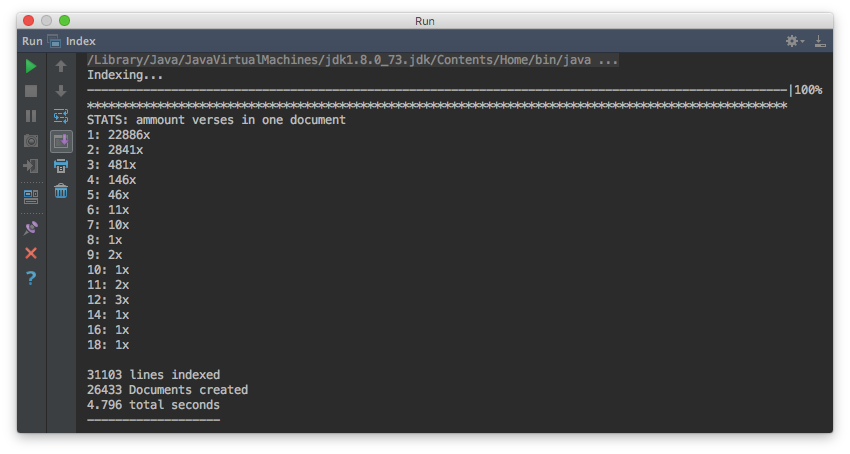
\includegraphics[width=1.0\textwidth]{images/3-realization/indexing_screenshot.png}
	\caption{Screenshot der Indexierung}
\end{figure}


\newpage
\subsection{Index Optimierungen}

%\subsubsection{Satztrennung und Kontextberücksichtigung}
Die Optimierungen aus \secref{sec:documentOptimazing} wurden beide implementiert.

%\vspace{0.5em}
%\textit{Satztrennung}
%\vspace{0.5em}\\
\subsubsection{Satztrennung}
Bei der Satztrennungs-Optimierung wurde die Dokumentaufteilung wie folgt verändert:
Am Anfang war jeder Vers ein Dokument, was 31'103 \glspl{glos:documentLabel} ergab.
Nach der Optimierung waren es noch 26'433 \glspl{glos:documentLabel}, was einer Reduktion von 4'670 \glspl{glos:documentLabel}n entspricht.

Dabei wurden die Verse wie folgt zu neuen \glspl{glos:documentLabel}n zusammengefasst:
\begin{table}[H]
	\centering
	\small\renewcommand{\arraystretch}{1.4}
	\rowcolors{1}{tablerowcolor}{tablebodycolor}
	%
	\captionabove{Satztrennungs-Übersicht}
	%
	\begin{tabularx}{0.5\textwidth}{ R{0.2\linewidth} | Y }%
		\textbf{Verslänge pro Dokument} & \textbf{Anzahl Vorkommnisse}\\ \hline \hline
		1 & 22'886\\
		2 & 2'841\\
		3 & 481\\
		4 & 146\\
		5 & 46\\
		6 & 11\\
		7 & 10\\
		8 & 1\\
		9 & 2\\
		10 & 1\\
		11 & 2\\
		12 & 3\\
		14 & 1\\
		16 & 1\\
		18 & 1\\ \hline
		\textbf{Total} & \textbf{26'433}\\ \hline \hline
	\end{tabularx}
\end{table}

\newpage
\subsubsection{Exkurs: der "`forceMerge"'}
Der \gls{glos:indexLabel} der \glspl{glos:documentLabel} wird jeweils in verschiedene Segmente zusammengefasst, was unterschiedlichen \gls{glos:indexLabel}-Levels entspricht.

\begin{framed}
	\textbf{Beispiel}: Namensverzeichnisses mit verschiedenen Segmenten
	
	Die Gruppierung der \glspl{glos:documentLabel} erfolgt hierarchisch strukturiert.
	
	A -- C $\rightarrow$ A $\rightarrow$ Alexandra - Andrea
	
	Dabei entspricht jeder Teil einem Segment und jede Hierarchie einem \gls{glos:indexLabel}-Level.
\end{framed}

Mit der Methode $forceMerge(n)$ kann der \gls{glos:indexLabel} zu $n$ Segmenten zusammengefügt werden, was sich positiv auf die Suchzeit auswirkt. Allerdings ist diese Operation sehr kostenaufwändig und wird für grosse, dynamische \glspl{glos:indexLabel} nicht empfohlen.

Anscheinend wurde die Handhabung von mehreren Segmenten in Lucene in ab Version 3.5 deutlich verbessert, was die Option seltener notwendig macht.\footcite{LUCENE-rename_optimize_to_a_less_cool-sounding_name_ASF_JIRA_2016-05-08}

\begin{framed}
	\textbf{Einblick in die Index-Generierung mit und ohne \textit{forceMerge}}
	
	Für den relativ kleinen \gls{glos:indexLabel} der Bibel kann der \textit{forceMerge} problemlos durchgeführt werden.
	Die \gls{glos:indexingLabel} ohne \textit{forceMerge} dauert auf dem Testsystem durchschnittlich 3.2 Sekunden. Mit dem \textit{forceMerge} dauert der Prozess 3.5 Sekunden ($+0.3$ Sekunden).
	
	Obwohl  der \gls{glos:indexLabel} immer noch sehr schnell zusammengestellt wird, \ul{verlängert sich der Prozess mit \textit{forceMerge} um 9\%!}
	
	Daraus wird schnell ersichtlich, dass die Operation nur mit Vorsicht auf grosse \glspl{glos:indexLabel} angewandt werden darf.
\end{framed}


%\textit{Kontextberücksichtigung}
%\vspace{0.5em}\\
\subsubsection{Kontextberücksichtigung}
Die Kontextoptimierung wurde ebenfalls durchgeführt. Dies wirkt sich stark auf die \gls{glos:indexingLabel}s-Zeit aus.
Folgende Tabelle zeigt die Dauer der Indexierung auf, abhängig, ob der Kontext mit je drei benachbarten Versen \textit{indexiert \& gespeichert}, \textit{nur indexiert} oder \textit{gar nicht} in den Index aufgenommen worden ist.
Ausserdem ist der prozentuale Zeitanstieg für die \gls{glos:indexingLabel} mit \textit{forceMerge} je Indextyp angegeben.
\begin{table}[H]
	\centering
	\small\renewcommand{\arraystretch}{1.4}
	\rowcolors{1}{tablerowcolor}{tablebodycolor}
	%
	\captionabove{Indexierungs-Zeit: abhängig der Feldgrösse und \textit{forceMerge (fm)}}
	%
	\begin{tabularx}{\textwidth}{ R{0.2\linewidth} || R{0.1\linewidth} | R{0.1\linewidth} || R{0.09\linewidth} | R{0.09\linewidth} || R{0.09\linewidth} | Y || }%
		 & \multicolumn{2}{l||}{\textbf{index. \& gespeichert}} & \multicolumn{2}{l||}{\textbf{indexiert}} & \multicolumn{2}{l||}{\textbf{ohne}}\\
		& \textit{ohne fm} & \textit{mit fm} & \textit{ohne fm} & \textit{mit fm} & \textit{ohne fm} & \textit{mit fm}\\ \hline \hline
		Messung 1 (s) & 4.8 & 6.5 & 4.7 & 6.9 & 3.3 & 3.5\\
		Messung 2 (s) & 5.0 & 6.8 & 4.85 & 7.6 & 3.1 & 3.5\\
		Messung 3 (s) & 5.3 & 6.3 & 4.9 & 6.4 & 3.1 & 3.6\\
		Messung 4 (s) & 5.0 & 7.6 & 4.8 & 6.3 & 3.2 & 3.5\\ \hline \hline
		\O \, (s) & \textbf{5.0} & \textbf{6.8} & \textbf{4.8} & \textbf{6.8} & \textbf{3.2} & \textbf{3.5}\\
		Zeitanstieg (\%)& & \textbf{+36} &  & \textbf{+42} &  & \textbf{+9}\\ \hline
		Index Grösse (MB) & \multicolumn{2}{r||}{9.1} & \multicolumn{2}{r||}{7.4} & \multicolumn{2}{r||}{3.8}\\
	\end{tabularx}
\end{table}

\vspace{0.5em}
\textit{Auswertung der Kontextberücksichtigung}
\vspace{0.5em}\\
Die Kontextoptimierung funktioniert grundsätzlich wie geplant. Auf Grund der beschränkten Zeit des Projektes kann der genaue Effekt dieser Optimierung nicht genauer bemessen werden.

Ein Nachteil der Kontextberücksichtigung ist, dass Verse, die den Suchbegriff nur in den Nachbarversen beinhalten trotzdem in der Resultat Liste erscheinen.
Durch die niedrige Gewichtung (auch Boost genannt) von ungefähr 0.7, erscheinen diese Verse nach den Treffern, jedoch wird dadurch trotzdem die Precision, bei der die Anzahl Ergebnisse verwendet wird, negativ beeinflusst.

Bei einer Suchmaschine mit Ranking, spielt dieses Total der Ergebnisse keine zentrale Rolle, weil der Nutzer oft nur einen kleinen Teil der Ergebnismenge anschaut.
Somit ist der genannte Nebeneffekt vertretbar.
Zudem kann es sogar vorkommen, dass der Benutzer ausschliesslich auf Grund der Vielfalt von indexierbarem Inhalt doch ein Ergebnis findet.
Ganz nach dem Grundsatz: lieber ein Ergebnis mit tiefem Score, als kein Ergebnis.


\subsection{Indexierte Felder}
Für jedes Feld das in den \gls{glos:indexLabel} aufgenommen wird, können zwei Eigenschaften definiert werden: ob das Feld \textit{indexiert} werden soll und ob es \textit{persistiert} werden soll.
Nach indexierte Werten kann gesucht werden. Persistierte Werte stehen für jeden Treffer vollständig zur Verfügung.
%Um Felder im \gls{glos:indexLabel} aufzunehmen, können je zwei Eigenschaften definiert werden: soll das Feld indexiert werden und soll das Feld vollständig persistiert werden.

Nach allen indexierten Feldern kann anschliessend gesucht werden. Persistierte Felder können ausgelesen werden und so kontextspezifische Informationen wie Referenzen und Stellenangaben beinhalten.

Im Index soll lediglich der Vers-Text (\textit{content}) indexiert werden.
Dazu müssen folgende weitere Referenzinformationen mit abgelegt werden: \textit{id}, \textit{book}, \textit{chapter}, \textit{verse}.

Zusätzlich für den Versuch der Kontext Optimierung (siehe \secref{sec:contextOptimaze}) sollen die Nachbarverse ebenfalls indexiert werden. Sie werden ins Feld \textit{context} gespeichert und ebenfalls indexiert.


\section{Suche}
\subsection{Anfrage-Syntax}
Für die Suche kann die vollständige Lucene Query Syntax verwendet werden. Mögliche Anfragen sind auf der Website aufgelistet.\footcite{Lucene_Query_Syntax_Lucene_Tutorial_2016-05-09}

Für den Suchbegriff müssen die gleichen Optimierungen wie für die \gls{glos:indexingLabel} (\secref{sec:indexing}) angewendet werden, so dass eine einheitliche Ausgangslage besteht.

\section{Features}
Obwohl die Suchmaschine nur via \gls{cliLabel} bedient werden kann, sollen trotzdem grundlegende Features zur Verfügung gestellt werden:
\begin{itemize}[noitemsep]
	\item \textit{Paging}:
	Die Suchresultate werden gemäss dem \gls{glos:rankingLabel} aufgelistet. Es soll das Total der Ergebnisse angezeigt werden. Anschliessend folgen jeweils Seiten mit je 10 Ergebnissen, durch die navigiert werden kann.
	Die Navigation bietet die Möglichkeit, zur nächsten, zur vorgängigen und zu einer bestimmten Seite zu wechseln.
	
	\item \textit{Highlighter}:
	Um das Ergebnis angenehm auswerten zu können, werden die Treffer farblich hervorgehoben, falls dies vom Terminal unterstützt wird.

	\item \textit{Suggest}:
	Falls ähnlich geschriebene Begriffe im Index vorkommen, soll eine Funktion "`Did you mean:"' den ähnlichsten Begriff anzeigen.
	
\end{itemize}

\vfill
\begin{figure}[H]
	\centering
	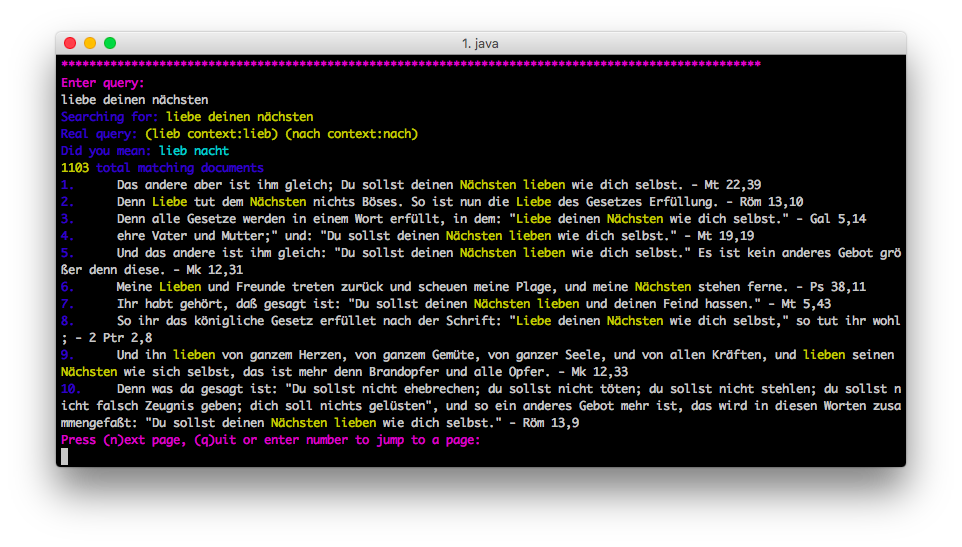
\includegraphics[width=1.0\textwidth]{images/3-realization/searching_screenshot.png}
	\caption{Screenshot der Suchmaschine inkl. Ergebnisse}
\end{figure}

%\section{Index Analyse mit Luke}
%\todo{Analyse mit Luke bei genügend Zeit}
